% The norm fibres x^2+y^2=a in F_7^2: one point for a=0 and six 8-point conics.
\documentclass[tikz,border=8pt]{standalone}
\usepackage{amsmath,amssymb}
\definecolor{n0}{HTML}{333333}
\definecolor{n1}{HTML}{2166AC}
\definecolor{n2}{HTML}{1B7837}
\definecolor{n3}{HTML}{762A83}
\definecolor{n4}{HTML}{D6604D}
\definecolor{n5}{HTML}{F4A582}
\definecolor{n6}{HTML}{92C5DE}
\begin{document}
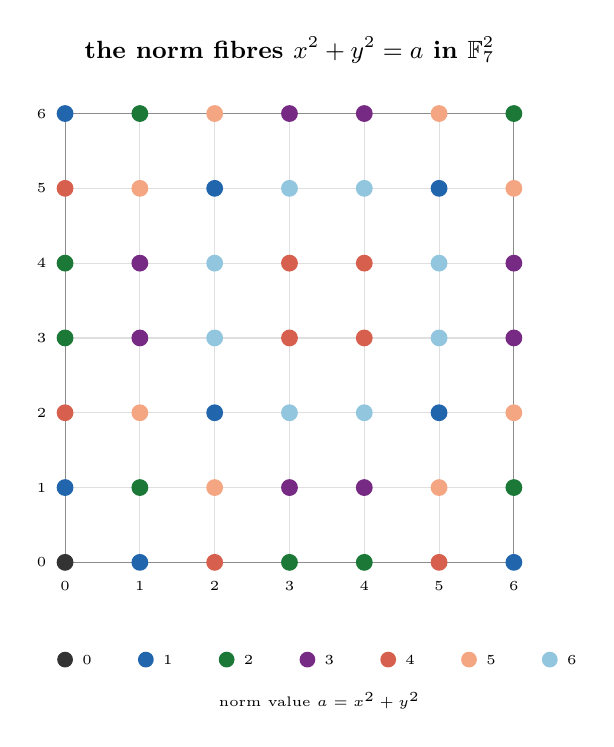
\begin{tikzpicture}[scale=0.95]
  \draw[gray!25] (0,0) grid (6,6);
  \draw[black!45] (0,0) rectangle (6,6);
  \foreach \x in {0,...,6} {%
    \node[font=\tiny,below] at (\x,-0.12) {\x};%
    \node[font=\tiny,left] at (-0.12,\x) {\x};%
    \foreach \y in {0,...,6} {%
      \pgfmathtruncatemacro{\a}{mod(\x*\x+\y*\y,7)}%
      \fill[color=n\a] (\x,\y) circle (3.2pt);%
    }%
  }
  \node[font=\small\bfseries] at (3,6.85) {the norm fibres $x^2+y^2=a$ in $\mathbb F_7^2$};
  % legend
  \foreach \a in {0,...,6} {%
    \fill[color=n\a] ({\a*1.08},-1.30) circle (3pt);%
    \node[font=\tiny,right] at ({\a*1.08+0.10},-1.30) {$\a$};%
  }
  \node[font=\tiny] at (3.4,-1.85) {norm value $a=x^2+y^2$};
\end{tikzpicture}
\end{document}
